% SIAM Article Template
\documentclass[onefignum,onetabnum]{siamart190516}


% Information that is shared between the article and the supplement
% (title and author information, macros, packages, etc.) goes into
% ex_shared.tex. If there is no supplement, this file can be included
% directly.

\usepackage{lipsum}
\usepackage{amsfonts}
\usepackage{graphicx}
\usepackage{amssymb}
\usepackage{epstopdf}
\usepackage{multirow}
\usepackage{mathrsfs}
\usepackage{algorithmic}
\ifpdf
  \DeclareGraphicsExtensions{.eps,.pdf,.png,.jpg}
\else
  \DeclareGraphicsExtensions{.eps}
\fi

% Add a serial/Oxford comma by default.
\newcommand{\creflastconjunction}{, and~}

% Used for creating new theorem and remark environments
\newsiamremark{remark}{Remark}
\newsiamremark{hypothesis}{Hypothesis}
\newsiamremark{problem}{Problem}
\crefname{hypothesis}{Hypothesis}{Hypotheses}
\newsiamthm{claim}{Claim}

%%%%%%%%%%%%%%%%%%%%%%%%%%%%%%%%%%%%%%%%%%%
% Equation
\newcommand{\be}{\begin{equation}}
\newcommand{\ee}{\end{equation}}

%%%%%%%%%%%%%%%%%%%%%%%%%%%%%%%%%%%%%%%%%%%
% bold symbols
\newcommand{\bq}{{\bf q}}
\newcommand{\bp}{{\bf p}}

\newcommand{\bH}{{\bf H}}
\newcommand{\bL}{{\bf L}}

%%%%%%%%%%%%%%%%%%%%%%%%%%%%%%%%%%%%%%%%%%%
% text symbols
\newcommand{\U}{\textup{U}}

%%%%%%%%%%%%%%%%%%%%%%%%%%%%%%%%%%%%%%%%%%%
% mathbb symbols
\newcommand{\IH}{\mathbb{H}}
\newcommand{\IN}{\mathbb{N}}
\newcommand{\IR}{\mathbb{R}}
\newcommand{\IX}{\mathbb{X}}


%%%%%%%%%%%%%%%%%%%%%%%%%%%%%%%%%%%%%%%%%%%
% mathbf symbols
\newcommand{\bn}{{\bf n}}
\newcommand{\bu}{{\bf u}}
\newcommand{\bv}{{\bf v}}
\newcommand{\bx}{{\bf x}}
\newcommand{\by}{{\bf y}}
\newcommand{\bxi}{\boldsymbol{\xi}}
\newcommand{\bgamma}{\boldsymbol{\gamma}}

%%%%%%%%%%%%%%%%%%%%%%%%%%%%%%%%%%%%%%%%%%%
% mathfs symbols
\newcommand{\fA}{\mathsf{A}}
\newcommand{\fI}{\mathsf{I}}
\newcommand{\fL}{\mathsf{L}}

\newcommand{\fm}{\mathsf{m}}
\newcommand{\fM}{\mathsf{M}}

\newcommand{\fQ}{\mathsf{Q}}
\newcommand{\fX}{\mathsf{X}}



%%%%%%%%%%%%%%%%%%%%%%%%%%%%%%%%%%%%%%%%%%%
% mathcal symbols
\newcommand{\mA}{\mathcal{A}}
\newcommand{\mC}{\mathcal{C}}
\newcommand{\mD}{\mathcal{D}}
\newcommand{\mI}{\mathcal{I}}
\newcommand{\mK}{\mathcal{K}}
\newcommand{\mP}{\mathcal{P}}
\newcommand{\mQ}{\mathcal{Q}}
\newcommand{\mR}{\mathcal{R}}
\newcommand{\mS}{\mathcal{S}}
\newcommand{\mX}{\mathcal{X}}
\newcommand{\mV}{\mathcal{V}}
\newcommand{\mW}{\mathcal{W}}

%%%%%%%%%%%%%%%%%%%%%%%%%%%%%%%%%%%%%%%%%%%
% Mathfrak
\newcommand{\fu}{\mathfrak{u}}

%%%%%%%%%%%%%%%%%%%%%%%%%%%%%%%%%%%%%%%%%%%
% Operators
\newcommand{\card}{\operatorname{card}}
\newcommand{\loc}{{\operatorname{loc}}}
\newcommand{\bcurl}{\operatorname{\bf{curl}}}
\newcommand{\divg}{\operatorname{div}}
\newcommand{\inc}{\operatorname{inc}}
\newcommand{\scat}{\operatorname{scat}}

\newcommand{\DL}{\mathsf{DL}}
\newcommand{\SL}{\mathsf{SL}}

\newcommand{\fR}{\mathsf{R}}

%%%%%%%%%%%%%%%%%%%%%%%%%%%%%%%%%%%%%%%%%%%
% Temporary commands
\newcommand{\todo}[1]{{\color{red}[#1]}}
\newcommand{\pe}[1]{{\color{blue}[#1]}}


% Sets running headers as well as PDF title and authors
\headers{Implementation of Multiple-Trace-Methods}{T. Betcke, X. Claeys, P. Escapil-Inchausp\'{e}, C. Jerez-Hanckes}

% Title. If the supplement option is on, then "Supplementary Material"
% is automatically inserted before the title.
\title{Practical implementations of multiple-trace methods for acoustic and electromagnetic scattering in complex media\thanks{Submitted to the editors DATE.
\funding{This work was funded by BLA BLA BLA.}}}

% Authors: full names plus addresses.
\author{Timo Betcke\thanks{University College London, London, UK (\email{t.betcke@ucl.ac.uk}).}
\and Xavier Claeys\thanks{Sorbonne Universit\'es, UPMC Univ Paris 06, CNRS, INRIA, UMR 7598, Laboratoire Jacques-Louis Lions, \'Equipe Alpines, 4, place Jussieu 75005, Paris, France
  (\email{claeys@ljll.math.upmc.fr}).}
\and Paul Escapil-Inchausp\'{e}\thanks{School of Engineering, Pontificia Universidad Cat\'olica de Chile, Santiago, Chile (\email{pescapil@uc.cl}).}
\and Carlos Jerez-Hanckes\thanks{Faculty of Engineering and Sciences, Universidad Adolfo Ib\'a\~{n}ez, Santiago, Chile (\email{carlos.jerez@uai.cl}).}}

\usepackage{amsopn}
\DeclareMathOperator{\diag}{diag}
% Optional PDF information
\ifpdf
\hypersetup{
  pdftitle={Practical implementations of multiple-trace methods for acoustic and electromagnetic scattering in complex media},
  pdfauthor={T. Betcke, X. Claeys, P. Escapil-Enchausp\`{e}, C. Jerez-Hanckes}
}
\fi

% The next statement enables references to information in the
% supplement. See the xr-hyperref package for details.

%\externaldocument{ex_supplement}

% FundRef data to be entered by SIAM
%<funding-group specific-use="FundRef">
%<award-group>
%<funding-source>
%<named-content content-type="funder-name"> 
%</named-content> 
%<named-content content-type="funder-identifier"> 
%</named-content>
%</funding-source>
%<award-id> </award-id>
%</award-group>
%</funding-group>

\begin{document}

\maketitle
% REQUIRED
\begin{abstract}
We consider solving the acoustic and electromagnetic scattering problems ...
\end{abstract}

% REQUIRED
\begin{keywords}
  example, \LaTeX
\end{keywords}

% REQUIRED
\begin{AMS}
  68Q25, 68R10, 68U05
\end{AMS}

\section{Introduction}
\label{sec:introduction}

\begin{itemize}
    \item
    \item Background of MTF formulations / literature overview. \pe{Implementation is challenging. } 
    \item Previous work, basic definitions
    \item Purpose of the paper 
    \item Overview of sections
\end{itemize}
In the sequel, we consider the time-harmonic acoustic in (resp.~electromagnetic) scattering from a $M$-composite object, $M \in \IN_0$, $\IN_0:=\{0,1,\cdots\}$ given by a partition of the free space as $\IR^3$,  with $\Omega_i \cap \Omega_j = \varnothing$, $i,j \in \{0,\cdots,M\}$, where $\Omega_m$'s, $m\in \{1,\cdots,M\}$ are connected and bounded Lipschitz domains. In what follow, $i,j$ indices will always refer to domains while we reserve $m$ index for scatterers. Next, we define the normal vector field $\bn_i$ pointing toward the exterior of $\Omega_i$, together with $\Gamma_i:=\partial \Omega_i$ the boundary of each domain and the interfaces $\Gamma_{ij}:=\Gamma_i\cap
\Gamma_{j}$, with the normal pointing from domain $i$ to $j$. Therefore, we introduce the skeleton as:
\be
\Sigma:= \bigcup_{i=0}^M \Gamma_i=\bigcup_{0\leq i \leq j \leq M}\overline{\Gamma}_{ij}.
\ee
To finish, we illustrate a $4$-composite object in \Cref{fig:skeleton}. We decide to highlight the boundary of domain $\Omega_3$ (in green) as well as the interface between domains $\Omega_2$ and $\Omega_1$ (in red). Furthermore, we  represent the skeleton $\Sigma$ in blue.
\begin{figure}[ht]
\center
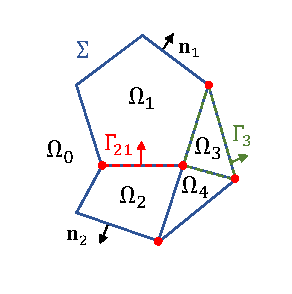
\includegraphics[width=.5\textwidth]{figs/skeleton.pdf}
\caption{Representation of a $4$-composite object.}
\label{fig:skeleton}       
\end{figure}
Having described the domains and their interfaces, we are ready to introduce the tools to settle the transmission problem.
 
\section{Transmission  problem}\label{sec:problem}
Let us consider a $M$-composite object (refer to \Cref{sec:introduction}) and characterize each domain as a medium with constant physical parameters. These are for each medium $\mu_i,c_i>0$ for acoustic scattering --representing the density and speed of sound in the medium, and $\epsilon_i,\mu_i>0$ for electromagnetic scattering --representing the permittivity and permeability in the medium.

To set the transmission problem for both acoustic and electromagnetic cases, we need to introduce a number of mathematical tools. These are described extensively in \Cref{tab:ParametersSetting}.

\begin{table}[ht]
\renewcommand\arraystretch{1.8}
\begin{center}
%\resizebox{9cm}{!} {
\begin{tabular}{
|c|c|c|}\hline
&  Acoustics & Electromagnetics \\ \hline
%&  \includegraphics[width=0.35\linewidth]{figs/pec_a.pdf} &  \includegraphics[width=0.35\linewidth]{figs/pec_e.pdf}\\ \hline
{\bf Parameters} & $\mu_i,c_i>0$, $k_i := \omega  / c_i$ & $\mu_i,\epsilon_i>0$, $k_i := \omega \sqrt{\epsilon_i \mu_i}$\\\hline
$\fL_{k_i}$ & $- \Delta\U^i  - k^2\U^i$&  $-\bcurl \bcurl\U^i - k_i^2 \U^i $ \\ \hline
 \multirow{2}{*}{{\bf Traces}} & $\gamma^i_0 \U^i:= \U^i|_{\Gamma_i}$ & $\gamma^i_0\U^i  := \U^i|_{\Gamma_i} \times \bn_i$ \\
  & $\gamma^i_1 \U^i:= \bn_i \cdot \nabla \U^i|_{\Gamma_i}$  & $\gamma^i_1 \U^i: = \frac{1}{\imath k_i}(\bn_i \times \bcurl \U^i|_{\Gamma_i})$\\\hline
  \multirow{2}{*}{$\fu_i$}  & \multirow{2}{*}{$\Big(\gamma^i_0 \U^i, \frac{1}{\mu_i}\gamma^i_1\U^i\Big)$} &  \multirow{2}{*}{$\Big(\gamma^i_0 \U^i, \frac{k_i}{\mu_i}\gamma^i_1\U^i\Big)$} \\
  & & \\\hline
  \multirow{2}{*}{$\IH(\Gamma_i)$} & \multirow{2}{*}{$H^{-1/2}(\Gamma_i)\times H^{1/2}(\Gamma_i) $} & \multirow{2}{*}{$\bH_\times^{-1/2}(\divg_\Gamma, \Gamma_i)^2$ }\\
  & & \\\hline
  RC & Sommerfeld &  Silver-M\"uller \\ \hline
 \end{tabular}%}
\caption{Overview of the proposed notations for each domain $\Omega_i$ with exterior normal field $\bn_i$.}
\label{tab:ParametersSetting}
\end{center} 
\end{table}  

In first row, having defined each medium, we set the wavenumber $k_i$. In second row, we define the respective Helmholtz (resp.~Maxwell) equation operator $\fL_{k_i}$. 

In third row, provided a smooth enough scalar field (resp.~vector field) $\U_i$ defined over $\Omega_i$, we introduce the Dirichlet and Neumann traces $\gamma^i_0\U^i$ and $\gamma^i_1\U^i$, and set $\gamma^i \U^i := (\gamma^i_0 \U^i,\gamma^i_1 \U^i)$. Traces are function to $\bn_i$ the normal exterior field. Similarly, for any $\U^i_c$ defined over $\IR^3 \backslash \overline{\Omega_i}$, we introduce the complement traces $\gamma^i_c \U^i_c$. The latter allows to define trace jumps and averages:
\be
\{\gamma^i \U^i\}_{\Gamma_i}:= \big(\gamma^i \U^i - \gamma_c^i \U^i_c\big) \textup{, and } [\gamma^i\U^i]_{\Gamma_i}:= \frac{1}{2}\big(\gamma^i\U^i + \gamma^i_c\U^i_c\big).
\ee

In fourth row we set $\fu_i$ the scaled traces which will be the unknowns in multi-trace formulations, along with their associated Sobolev function space for each $\Gamma_i$ in fifth row (see \cite[Section 6.2]{claeys2012multi} and \cite[Section 2.2]{buffa2003galerkin}). In last row, we show the radiation condition for each problem (refer to \cite[Equations 2.2.5 and Theorem 5.2.2]{Nedelec}).

%\begin{remark}[Physical meaning of $\fu_i$]
%\todo{todo, explain how to recover physical quantities from $\fu_i$}
%\todo{Add a remark concerning formulation for $\mathbf{e} \times \bn $ and $\mathbf{h} \times \bn$ as the unknowns}
%\end{remark}

Next, we describe the boundary transmission conditions at each interface in  first row of \Cref{tab:TransmissionConditions}. These are reformulated in terms of unknowns $\fu_i,\fu_j$ in second row, along with the expression of the transmission matrix $\mQ$ in  third row.

In last row, we represent the adapted Sobolev tilde spaces for those transmission conditions (see \cite[Section 5.1]{claeys2014novel} \todo{def tilde for Maxwell}).
\begin{table}[ht]
\renewcommand\arraystretch{1.7}
\begin{center}
\resizebox{13cm}{!} {
\begin{tabular}{
|c|c|c|}\hline
&  Acoustics & Electromagnetics \\ \hline
\multirow{2}{*}{TC$(\U^i,\U^j)$} & $\U^i|_{\Gamma_{ij}} =\U^j|_{\Gamma_{ji}}$ & $\U^i|_{\Gamma_{ij}} \cdot \bn_i = - \U^j|_{\Gamma_{ji}}\cdot \bn_j $\\
& $\mu_i^{-1}\bn_i \cdot \nabla \U^i|_{\Gamma_{ij}}  = -\mu_j^{-1} \bn_j \cdot \nabla \U^j|_{\Gamma_{ji}}$ & $\mu_i^{-1} (\bn_i \times \bcurl \U^i|_{\Gamma_{ij}}) = -\mu_j^{-1} (\bn_j \times \bcurl \U^j|_{\Gamma_{ji}}) $\\\hline
 \multirow{2}{*}{TC$(\fu^i,\fu^j)$}&\multirow{2}{*}{$\fu_i|_{\Gamma_{ij}}=\mQ \fu_j|_{\Gamma_{ji}}$} &\multirow{2}{*}{$\fu_i|_{\Gamma_{ij}}=\mQ \fu_j|_{\Gamma_{ji}}$} \\
 &&\\\hline
 \multirow{3}{*}{$\mQ$}&\multirow{3}{*}{$\begin{pmatrix} +1 & 0 \\ 0 & -1 \end{pmatrix}$} &\multirow{3}{*}{$\begin{pmatrix} -1 & 0 \\ 0 & -1 \end{pmatrix}$} \\
 &&\\ 
&&\\\hline
 \multirow{2}{*}{$\widetilde{\IH}(\Gamma_{ij})$} &\multirow{2}{*}{$\tilde{H}^{-1/2}(\Gamma_{ij})\times \tilde{H}^{-1/2}(\Gamma_{ij}) $} &\multirow{2}{*}{ $\widetilde{\bH}_\times^{-1/2}(\divg_\Gamma, \Gamma)^2$} \\
 &&\\\hline
\end{tabular}}
\caption{Overview of the transmission conditions at interfaces with their adapted function spaces.}
\label{tab:TransmissionConditions}
\end{center} 
\end{table} 

Lastly, we introduce in \Cref{prob:transmission} the $M$-composite transmission problem and set $\U \equiv [\U_0,\cdots,\U_M]$. Notice that the incident field is defined over $\Omega_0$ and can be identified as $\U^{\inc} \equiv \U^{0,\inc}\equiv [\U^{\inc} ,0,\cdots,0]$:
\begin{problem}[$M$-composite transmission problem]\label{prob:transmission}Given an incident wave $\U^{\inc}$ with  $\fL_{k_0}\U^{\inc}=0$ in $\Omega_0$, seek $\U := \U^{\inc} + \U^{\scat}$ solution of:
$$
\left\{
\begin{array}{lll}
\fL_{k_i}\U^i  = 0&\textup{ in } \Omega_i,\\
\noalign{\vspace{3pt}}
  \textup{TC}(\U^i,\U^j)&\textup{ on } \Gamma_{ij},\\
  \noalign{\vspace{3pt}}
    \textup{RC}(\U^{\scat}).
\end{array}
\right.
$$
\end{problem}
This problem is known to be well-posed \cite[Theorem 1.2]{claeys2012multi}.
\section{Boundary Integral Operators for acoustic and electromagnetic scattering}\label{sec:BIOs}
\subsection{Single domain}\label{subs:BIOsSingleDomain}
To begin with, we restrict ourselves to a single bounded Lipschitz domain $\Omega$ with boundary $\Gamma$ and exterior normal field $\bn$. The definitions will further apply to all $\Omega_i$'s. To begin with, we introduce the fundamental solution $G_k(\bx,\by)$ of the Helmholtz equation for $k>0$ with $\|\cdot\|_2$ the Euclidean norm:
\be
G_k(\bx,\by) :=\dfrac{\imath}{4\pi}\dfrac{ \exp (\imath k \|\bx-\by\|_2)}{\|\bx-\by\|_2} .
\ee
With this, we introduce the acoustic single- and double-layer potentials for a boundary scalar field $\phi$ at $\bx \in \IR^3\backslash \Gamma$:
\begin{align*}
\SL_k (\phi) (\bx) &:= \int_\Gamma G_k (\bx,\by) \phi(\by) d\Gamma(\by), \\
\DL_k (\phi) (\bx) &:= \int_\Gamma \frac{\partial}{\partial \bn_\by}  G_k (\bx,\by) \phi(\by) d\Gamma(\by).
\end{align*}
Consequently, we define the following boundary integral operators:
\be
\begin{array}{lll}
\mV_k &: H^{-1/2}(\Gamma) \to H^{1/2}(\Gamma), & \mV_k := \{\gamma_0 \}_\Gamma \circ \SL_k,\\
\mK_k &: H^{1/2}(\Gamma) \to H^{1/2}(\Gamma), & \mK_k := \{ \gamma_0 \}_\Gamma \circ \DL_k,\\
\mK'_k &: H^{-1/2}(\Gamma) \to H^{-1/2}(\Gamma), & \mK'_k := \{ \gamma_1 \}_\Gamma \circ \SL_k,\\
\mW_k &: H^{1/2}(\Gamma) \to H^{-1/2}(\Gamma), & \mW_k := -\{\gamma_1\}_\Gamma \circ \DL_k.
\end{array}
\ee
Likewise, we introduce the electromagnetic counterparts of these potentials for a boundary vector field $\phi$ at $\bx \in \IR^3\backslash \Gamma$:
\begin{align*}
\SL_k (\phi) (\bx) &:= \imath k \int_\Gamma G_k (\bx,\by) \phi(\by) d\Gamma(\by)-\frac{1}{\imath k}\nabla_\bx \int_\Gamma \nabla_\by \cdot \phi(\by)G_k(\bx,\by)d\Gamma(\by),\\
\DL_k (\phi) (\bx) &:=\nabla_\bx \times \int_\Gamma \phi (\by) G_k(\bx,\by)d\Gamma (\by).
\end{align*}
In a similar fashion, we introduce the boundary integral operators:
\be
\begin{array}{lll}
\mC_k &: \bH_\times^{-1/2}(\divg_\Gamma, \Gamma) \to \bH_\times^{-1/2}(\divg_\Gamma, \Gamma), & \mC_k := \{\gamma_0 \}_\Gamma \circ \SL_k,\\
\mS_k &: \bH_\times^{-1/2}(\divg_\Gamma, \Gamma) \to \bH_\times^{-1/2}(\divg_\Gamma, \Gamma), & \mS_k := \{ \gamma_0 \}_\Gamma \circ \DL_k.
\end{array}
\ee

With this at hand, define the block Green's potential:
$$
\fR_k:= (-\DL_k ,\SL_k),
$$
\todo{Trace jumps in the representation formulas?}
We deduce the representation formulas for any \emph{radiating solution} (see \cite[Theorem 2.2]{claeys2012multi}):
\be
\label{eq:representation_formula}
\U= \DL_k(\gamma_0 \U) - \SL_k(\gamma_1 \U) = \fR_k (\gamma\U)\textup{ in } \IR^3\backslash \Gamma,
\ee
and introduce the \emph{scaled multitrace operator} $\hat{\mA}$ as being
$$
\hat{\mA}_k : = \left(\begin{array}{cc}-\mK_k&\mu\mV_k\\\frac{1}{\mu}\mW_k & \mK'_k\end{array}\right)\quad \textup{and} \quad\hat{\mA}_k : = \left(\begin{array}{cc}\mC_k&\frac{\mu}{k}\mS_k\\-\frac{k}{\mu}\mS_k& \mC_k\end{array}\right)
$$
for acoustics and electromagnetics, respectively.

\begin{table}[ht]
\renewcommand\arraystretch{1.7}
\begin{center}
%\resizebox{9cm}{!} {
\begin{tabular}{
|c|c|c|}\hline
&  Acoustics & Electromagnetics \\ \hline
\multirow{3}{*}{$\hat{\mA}_i$}& \multirow{3}{*}{$\left(\begin{array}{cc}-\mK_i&\mu\mV_i\\\frac{1}{\mu}\mW_i & \mK'_i\end{array}\right)$}&\multirow{3}{*}{ $\left(\begin{array}{cc}\mC_i&\frac{\mu}{k}\mS_i\\-\frac{k}{\mu}\mS_i & \mC_i\end{array}\right)$}\\
 &&\\
&&\\\hline
\multirow{3}{*}{$\hat{\mI}_{ij}$}& \multirow{3}{*}{$\left(\begin{array}{cc} -\mI_j&0\\0 & \mI_j\end{array}\right)$}&\multirow{3}{*}{ $\left(\begin{array}{cc} \mI_j&0\\0 & \mI_j\end{array}\right)$}\\
&&\\
&&\\ \hline
\end{tabular}%}
\caption{Description of the multitrace boundary integral operator.}
\label{tab:BoundaryOperators}
\end{center} 
\end{table} 
Having defined the multitrace operator, we introduce the identity operator in trace space $\mI$ and provide the interior and exterior Calder\'on identities: \todo{Use scaled version}
\be
\renewcommand\arraystretch{1.3}
\label{eq:cald}\begin{array}{cl}
\textup{(Interior)} &\gamma \U =  \left(\frac{1}{2}\mI+ \mA_k\right) \gamma \U = : \mP_{k} \gamma \U,\\
\textup{(Exterior)}   &\gamma_c \U_c =  \left(\frac{1}{2}\mI -\mA_k \right)\gamma_c \U_c =: \mP^c_{k} \gamma_c \U_c = (\mI - \mP_k)\gamma_c \U_c.
\end{array}
\ee
\subsection{$M$-composite domain}\label{subs:BIOsMultipleDomain}We now consider a $M$-composite object for any $M \in \IN_0$. Similar to \Cref{subs:BIOsSingleDomain}, we introduce the respective boundary and potential operators, denoted with $i$ subscripts (instead of $k$ subscripts). Moreover, we set the identity operator $\mI_i$, and introduce the restriction $\mI_{ij} :\IH(\Gamma_i) \to \IH(\Gamma_{ij})$:
\begin{align*}
\mI_{ij} &: = \chi_{ij} \mI_i= \chi_{ij} \mI_j,
\end{align*}
and we set the \emph{transfer operator} $\hat{\mX}_{ij}$ as being
$$
\hat{\mX}_{ij} : = \left(\begin{array}{cc}  -\mI_{ij} & 0\\0 &  \mI_{ij}\end{array}\right)\quad \textup{and} \quad\hat{\mX}_{ij} : = \left(\begin{array}{cc}  \mI_{ij} & 0\\0 &  \mI_{ij}\end{array}\right)
$$
for acoustics and electromagnetics, respectively.


We finally introduce $\hat{\fA}:= \textup{diag}(\hat{\mA}_i)$ and $\hat{\fX}:= (\hat{\fX}_{ij})_{i,j = 1}^M$.We arrive at the final formulation for the local MTF.
\begin{problem}\label{pb:MTF}
Seek $\bu \in \IH$ such that
\be 
(2\hat{\fA} - \hat{\fX}) \bu = - 2\bu_0^\textup{inc}.
\ee 
\end{problem}
\begin{proof}For $\Omega_0$, one has that that: 
\be 
\bu_0^\textup{sc} =  \left(\frac{1}{2}\mI_0+ \mA_0\right) \bu_0^\textup{sc}
\ee 
and 
\be 
\bu_0^\textup{inc} =  \left(\frac{1}{2}\mI_0- \mA_0\right) \bu_0^\textup{inc}
\ee 
hence
\begin{align*}
\bu_0 &= \frac{1}{2} \bu_0  + \mA_0 \bu_0^\textup{sc} - \mA_0 \bu_0^\textup{inc}\\
\frac{1}{2} \bu_0 &=   + \mA_0 \bu_0  - 2\mA_0 \bu_0^\textup{inc}\\
\left(\frac{1}{2}\mI_0 - \mA_0\right)\bu_0 & = -2 \mA_0 \bu_0^\textup{inc}= \bu_0^\textup{inc}
\end{align*}

We deduce the following relations: 
\begin{align*}
\left(\mA_{0} - \frac{1}{2}\mI_0  \right)\bu_0 &= -\bu_0^\textup{inc} \\
\left(\mA_{m}-\frac{1}{2}\mI_m  \right)\bu_m &= 0
\end{align*}
We rewrite transmission conditions as:
\begin{align*}
\bu_i &= \sum_{j \neq i} \bu_{i}|_{\Gamma_{ij}}\\
&=- \sum_{j\neq i} \bu_j|_{\Gamma_{ij}} \\
&=-\hat{\mI}_{ij} \bu_j|_{\Gamma_{ij}}= - \sum_{j \neq i} \hat{\mI}_{ji}\bu_j.
\end{align*}
\end{proof}

\begin{itemize}
\item Define integral operators and representation formulas for acoustics
\item Derive the Calderon operator as trace of representation formula
\item Galerkin discretisation of the operators
\item Introduce Maxwell operators, associated continuous and discrete spaces and briefly explain changes to acoustic case (formulation of Calderon operator for Maxwell)
\end{itemize}

\begin{itemize}
\item Show basic ideas of MTF
\item Discuss local vs global MTF
\item Describe preconditioning strategies
\end{itemize}

\section{Practical implementation of the MTF}

    \subsection{Grid handling for multiple-trace methods}
Multiple trace methods require to assemble multiple trace operators $\mA_i$ over all sub-domains $i$, and to evaluate the entries for the transfer operators $\mX_{ij}$ over all non-disjoint interfaces. This leads to implementation issues, provided that $\mA_i$ are related to closed sub-domains, whereas $\mX_{ij}$ are defined over the interfaces. This was remedied by following the proceeding that follows. 

To begin with, we introduce a locally quasi-uniform mesh \cite[Section 9.1]{steinbach2007numerical} for the skeleton as $\Sigma_h$. We assume that xx.

Concerning the definition of normal vector. We assume that for each triangle, it is pointing from $j$ to $i$ with $j>i$. The latter allows to define appropriately Physical Surfaces for GMRES. For the triple-point case, this leads to the definition of skeleton mesh $\Sigma_h := \tau_{20} \cup \tau_{10} \cup\tau_{21}$. In X we plot the mesh for xxx.
        \begin{itemize}
            \item Introduce skeleton meshes, identifying subsection of skeleton meshes
            \item Processing of elements for subdomains and fixing normal directions for each subdomain
        \end{itemize}

    \subsection{Space definitions on subdomains}
        \begin{itemize}
            \item Practical definition of spaces on subdomains (handling of boundary dofs, which to include, etc.)
            \item Correct trace spaces on single interfaces
        \end{itemize}
        
    \subsection{Assembly of multitrace and transfer operators}
    
        \begin{itemize}
            \item Multitrace operators need to take normal directions into account
            \item Multitrace transfer operators from one subdomain to another subdomain
            \item For transfer operators compute unions of elements, assemble operators on element unions, taking correct trace space definitions into acount
        \end{itemize}

    \subsection{Preconditioning}
    
        \begin{itemize}
            \item Adding preconditioning, give remarks on mass matrix inverses, Calderon preconditioners, etc.
        \end{itemize}
        
\section{Examples}

        \begin{itemize}
            \item Demonstrate interesting examples
            \item Preconditioning performance with growing wavenumber
            \item Error decay on interfaces vs. interior
            \item Comparison of local and global MTF
            \item Discuss parallel strategies
        \end{itemize}

\section{Conclusions}
\label{sec:conclusions}

Some conclusions here.

\section*{Acknowledgments}
\bibliographystyle{siamplain}
\bibliography{references}
\end{document}
